{
\subsection{Eksperimentsopstilling}
I \ref{chap_afproevning} er de optimale tærskelværdier fundet.
Idet denne hypotese blot kigger på frekvensen for brug af det gyldnesnit
mod andre snit, hvis eneste restriktion er at de skal have et fælles
forhold til det gyldnesnit.
Det er også fordelagtigt at maksimere antallet af andre snit, da det
giver et bedre grundlag for eksperimentet.
Afstanden mellem to snit er begrænset af margin defineret til at være
$2.4\%$\ref{margin}. 
Denne margin skal være tilstede på begge sider af et snit, så derfor vil
hvert snit fylde $(2.4*2)\%$.
Det maksimale antal af snit på et billede må altså være
$100/4.8=20.833$. Hvilket ses på denne figur \ref{snitogmargin}
\begin{figure}[ht]
	\begin{center}
		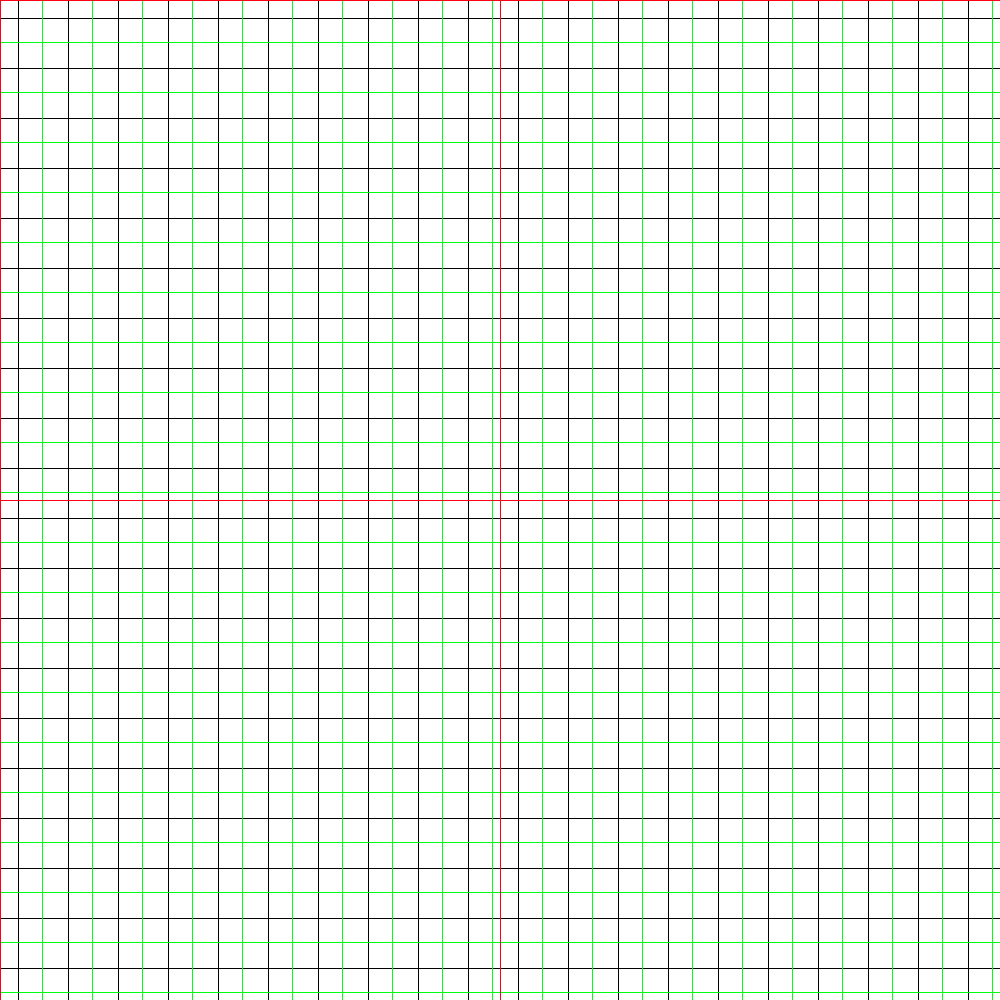
\includegraphics[scale=0.3]{afsnit/resultater/billeder/20_cuts_med_margin}
	\end{center}
	\caption{Sort:snittene, grøn: margins og rød er midten}
	\label{snitogmargin}
\end{figure}
Yderpunkterne $0.958$ og $0.518$ er problematiske, $0.958$'s margin
løber udover billedet, dvs. at den ren principielt går glip af at
detektere en masse interessante regioner.
$0.518$ lider af det modsatte problem, den kan potentielt fange
interessante regioner, på begge sider af midten.
For at være helt præcis så er det i $0.518$ tilfælde:\\
$1-0.518 = 0.482$
$0.518-0.482=0.036$\\
Hvilket er afstanden mellem de to snit.
Der er altså en stimmel på $0.05-0.036 = 0.014 = 1.4\%$ af billedet,
hvor interessante regioner bliver talt to gange.

\subsection{Systematisk fejl\label{program_bug}}
I den naive løsning findes en fejl i udtrækningen af regioner, som gør
at vi finder nogle af
regionerne flere gange. Denne fejl nævnt i afsnit
\ref{section_impBilledbehandling} og gennemgået i bilag
\ref{appendix_bug}. Det betyder, at de resultater vi fremviser for kørslen
af den naive løsning, ikke helt passer. For at give en indblik i, hvor
mange regioner der bliver fundet flere gange, har vi afprøvet programmet med
fejlen på 11 malerier, og sammenlignet dem med en kørsel, hvor fejlen er
rettet.

De 11 malerier er opstillet i tabel \ref{bug_tabel}, hvor de to første
kolonner er antal regioner fundet i billedet, uden og med fejl.  Tredje
kolonne er en procentsats for, hvor mange flere regioner der bliver
fundet, når den fejlende kode køres. Den procentvise spredning er $[60
\%,~377 \%]$, så de resultater vi får, kan være op til $377\%$ for høje.
Gennemsnitligt er der $172 \%$ flere regioner. Vi kan godt antage, at
antallet af regioner opgivet i resultaterne for den naive løsning, er
halv så store.

\begin{table}[!h]
    \centering
    \begin{tabular}{|l|c|c|c|}
        \hline
  Maleri  & Bug løst 		& Bug ikke løst		& Procentvis forskel\\\hline
        1   & 70 			& 112 				& 60 \% \\\hline
        2   & 27 			& 45 				& 67 \% \\\hline
        3	& 52 			& 98 				& 72 \% \\\hline
        4   & 84 			& 145 				& 73 \% \\\hline
        5	& 32 			& 57 				& 78 \% \\\hline
        6   & 88 			& 170 				& 93 \% \\\hline
        7   & 85 			& 201 				& 136 \% \\\hline
        8   & 78 			& 197 				& 153 \% \\\hline
        9   & 164 			& 554 				& 238 \% \\\hline
        10	& 16 			& 75 				& 368 \% \\\hline
        11	& 115 			& 548 				& 377 \% \\\hline
	Total	& 881			& 2202				& 172 \% \\\hline
	  \end{tabular}
    \caption[]{Tabel for antal fundne regioner i versionen med og uden
    fejlen som duplikerer regioner. Den sidste kolonne er hvor mange
    procent flere regioner der bliver fundet.}
    \label{bug_tabel}
\end{table}

\clearpage

\subsection{Resultater}
Vi har kørt vores analyse på $17,364$ malerier, men i vores resultater
sorterer vi $2,989$ af disse fra, da de kun er udsnit af et større maleri.
Som vist i tabel \ref{tabel_fjern_detaljer} herunder, er dette en nedgang
på $17.21$ procent og vi har $14,375$ brugbare resultater tilbage.

\begin{table}[H]
    \centering
    \begin{tabular}{r@{\ \ }p{12em}r|r@{.}l}
            & Analyserede malerier & $17,364$ & $100$ & $00\%$   \\
        $-$ & Udsnit af malerier   &  $2,989$ &  $17$ & $21\%$   \\\hline
            & Resultater           & $14,375$ &  $82$ & $79\%$
    \end{tabular}
    \caption[]{Udregning af brugbare resultater.}
    \label{tabel_fjern_detaljer}
\end{table}

Af de brugbare resultater, ser vi i tabel \ref{tabel_fordeling}, at der
i $91.43$ procent af malerierne er fundet mindst én region som ligger i
det gyldne snit. Vi kan derfor ikke afvise hypotese \ref{hypo_binaer}.

\begin{table}[H]
    \centering
    \begin{tabular}{r@{\ \ }p{12em}r|r@{.}l}
            & Positive resultater   & $13,143$ &  $91$ & $43\%$ \\
        $+$ & Negative resultater   &  $1,232$ &   $8$ & $57\%$ \\\hline
            & Resultater i alt      & $14,375$ & $100$ & $00\%$
    \end{tabular}
    \caption[]{Et positivt resultat beskriver et maleri, hvori der er
    fundet mindst én region, som ligger i det gyldne snit. Et negativt
    resultat er et maleri, hvori der ikke findes nogen regioner, som
    ligger i det gyldne snit.}
    \label{tabel_fordeling}
\end{table}

Vi vil gerne se på, hvordan fordelingen af fundne interessante regioner i
de fire gyldne snit ser ud. Fordelingen er vist i tabel
\ref{tabel_fire_snit}. Vi ser, at ingen af snittene afviger med mere end
$\pm10\%$ fra et andet og vi kan derfor ikke afvise hypotese
\ref{hypo_fire_g_snit}.

\begin{table}[H]
    \centering
    \begin{tabular}{r@{\ \ }p{12em}r|r@{.}l}
            & Regioner i snit 0   &  $41,087$ &  $24$ & $36\%$ \\
        $+$ & Regioner i snit 1   &  $42,400$ &  $25$ & $14\%$ \\
        $+$ & Regioner i snit 2   &  $45,038$ &  $26$ & $71\%$ \\
        $+$ & Regioner i snit 3   &  $40,125$ &  $23$ & $79\%$ \\\hline
            & Regioner i alt      & $168,650$ & $100$ & $00\%$
    \end{tabular}
    \caption[]{Forholdet mellem de interessante regioner fundet i de
    fire gyldne snit.}
    \label{tabel_fire_snit}
\end{table}

Vi undersøger nu, hvor mange af de brugbare resultater, som er forsynet
med dimensioner i databasen, således at vi kan undersøge, hvorvidt
lærredet er konstrueret som et gyldent rektangel. Udregningen i tabel
\ref{tabel_med_dimensioner} viser, at ud af de brugbare resultater,
mangler $2,410$ malerier dimensionerne, og vi har da $11,965$ malerier
tilbage at undersøge, for den gyldne ratio i lærredets dimensioner.

\begin{table}[H]
    \centering
    \begin{tabular}{r@{\ \ }p{14em}r|r@{.}l}
            & Resultater                     & $14,375$ & $100$ & $00\%$ \\
        $-$ & Resultater uden dimensioner    &  $2,410$ &  $16$ & $77\%$ \\\hline
            & Resultater med dimensioner     & $11,965$ &  $83$ & $23\%$
    \end{tabular}
    \caption[]{Brugbare resultater med dimensioner.}
    \label{tabel_med_dimensioner}
\end{table}

Vi ser nu, hvor mange af de $11,965$ malerier, der har, at dets lange
side, $L$, divideret med dets korte side, $K$, ligger i intervallet $G =
[1.57920117302, 1.65686680448] = \varphi \pm 2.4\%$. Tabel
\ref{tabel_real_dimensions} viser, at kun $3.99\%$ falder inden for
dette interval. Vi kan således afvise hypotese
\ref{hypo_golden_ractangle}.

\begin{table}[H]
    \centering
    \begin{tabular}{r@{\ \ }p{14em}r|r@{.}l}
            & $L/K \in G$                  &    $478$ &   $3$ & $99\%$ \\
        $+$ & $L/K \notin G$               & $11,487$ &  $96$ & $01\%$ \\\hline
            & Resultater med dimensioner   & $11,965$ & $100$ & $00\%$
    \end{tabular}
    \caption[]{Resultater med dimensioner, hvor disse er et gyldent
    rektangel med en afvigelse på $2.4\%$.}
    \label{tabel_real_dimensions}
\end{table}

\subsubsection{Antallet af fundne regioner over alle snit}
I alle $14,375$ malerier er der i alt fundet $1,578,611$ interessante
regioner. Vi har en middelværdi på $109.82$ med standardafvigelse på
$83.21$. I figur \ref{total_regions_plots} er vist nogle plots over
hvordan antallet af regioner fordeler sig i malerierne.  I figur
\ref{graf_total_regions_zoom}, hvor der ses bort fra $298$ malerier, som
ikke har nogen regioner. Regionerne i malerierne har en fordeling, der
kunne ligne en eksponentialfordeling, som vist i histogrammet i figur
\ref{hist_total_regions}. De observerede værdier fraviger dog noget fra
de teoretiske værdier.

\begin{figure}[!h]
    \centering
    \subfloat[]{
        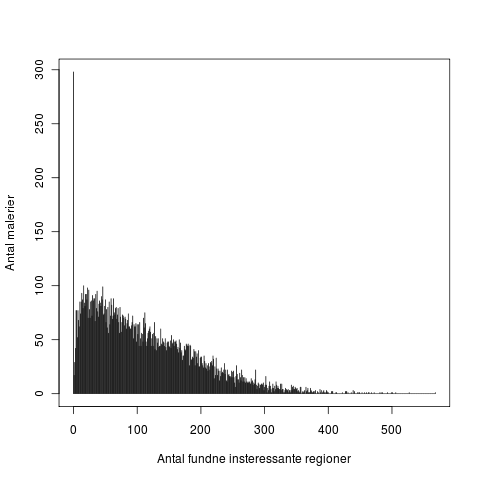
\includegraphics[width=0.49\textwidth]{afsnit/resultater/billeder/totalregions_var}
        \label{graf_total_regions_var}
    }
    \subfloat[]{
        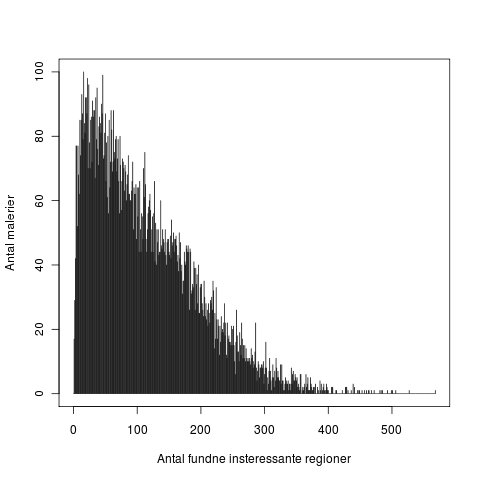
\includegraphics[width=0.49\textwidth]{afsnit/resultater/billeder/totalregions}
        \label{graf_total_regions_zoom}
    }\\
    \subfloat[]{
        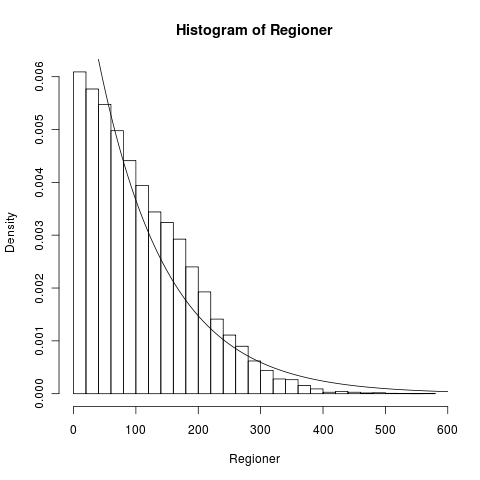
\includegraphics[width=0.62\textwidth]{afsnit/resultater/billeder/hist_totalregions}
        \label{hist_total_regions}
    }
    \caption[]{Fordelingen af fundne regioner på malerier.
    \textbf{\ref{graf_total_regions_var}:} Plot som viser hvor mange
    malerier, hvori der er fundet et vist antal interessante regioner
    over alle snit i maleriet.  \textbf{\ref{graf_total_regions_zoom}:}
    Samme plot som i figur \ref{graf_total_regions_var}, men hvor antal
    malerier uden regioner ikke er vist.
    \textbf{\ref{hist_total_regions}:} Histogram over antal fundne
    regioner, hvor en eksponentialfordeling med $\lambda = 1/109.82$ er
    indtegnet.}
    \label{total_regions_plots}
\end{figure}

Vi ser, at et maleri typisk har omkring $110$ interessante regioner i
alle snit. Her skal man være opmærksom på, at hver region meget vel
indgår fire gange. Vi ser, at der er et lille antal malerier, hvori der
bliver fundet rigtig mange regioner. Det tynder dog ud omkring
$380$ regioner, hvor antallet af malerier, med flere regioner,
forekommer mindre hyppigt.

\begin{table}[!h]
    \centering
    \begin{tabular}{|l|c|c|}
        \hline
            & Afvist & Ikke afvist  \\\hline
        1   &            & \checkmark   \\\hline
        2   &            & \checkmark   \\\hline
        3   & \checkmark &              \\\hline
        4   & \checkmark &              \\\hline
        5   &            & \checkmark   \\\hline
        6   & \checkmark &              \\\hline
        7   &            &              \\\hline
        8   &            &              \\\hline
        9   &            & \checkmark	\\\hline
    \end{tabular}
    \caption[]{Hypoteser i forhold til den naive kørsel.}
    \label{hypoteser_naiv}
\end{table}

}
% vim: set tw=72 spell spelllang=da:
